\documentclass[a4paper,12pt]{article} % format
\usepackage{fontspec} % fonts
\setmainfont{Times New Roman} % set font to TNR
\usepackage{tikz}
\usepackage{amsmath}

\usepackage{graphicx}

\usepackage{caption}

\captionsetup[figure]{labelsep=period}

\usepackage{csquotes}

\usepackage{amsmath}

\usepackage{titlesec} % title
\usepackage[english, russian]{babel} % languages
\usepackage{indentfirst} % for first paragraph indentation 

\usepackage{float} % for placing things where I want them to be

\renewcommand{\figurename}{Рисунок\_} 

\usepackage{setspace} % for space between lines

\usepackage[a4paper,
    left=3cm,
    right=2cm,
    top=2cm,
    bottom=2cm
    ]{geometry} % for margins

\usepackage{tocbibind}
\usepackage[style=gost-numeric,sorting=none, backend=biber]{biblatex}

\addbibresource{bib.bib}

\begin{document}

\addtocontents{toc}{\protect\setcounter{tocdepth}{-1}}


% Восстанавливаем уровень отображения
\addtocontents{toc}{\protect\setcounter{tocdepth}{2}}

\section{Аннотация}

Данный доклад фокусируется на методе численного интегрирования функции одной переменной c применением нейросетевого подхода. Суть нейросетевого подхода сводится к обучению нейросетевой модели аппроксимировать подынтегральную функцию и дальнейшему использованию параметров обученной нейросетевой модели для численного интегрирования данной функции на любом отрезке в области определения функции.

Применение нейросетевого подхода должно позволить повысить точность вычисления интегралов с большим количеством переменных. При вычислении значения численных интегралов функций многих переменных большинством классических численных методов (например, формула Симпсона, метод трапеций и др.) погрешность значения результатов увеличивается тем сильнее, чем больше число переменных подынтегральной функции. Растет также и сложность вычислений. Применение нейросетевого подхода должно решить данные проблемы, так как основные вычислительные ресурсы в нем тратятся на обучение сравнительной небольшой модели – многослойного перцептрона с одним скрытым слоем – один раз, а затем данную модель можно использовать для получения значений численных интегралов данной функции на разных отрезках много раз. При этом возможность гибкой настройки гиперпараметров обучаемой модели, теоретически позволяет достичь требуемой в прикладной задаче точности.

Данный доклад основан на бакалаврской работе, целью которой является разработка программного пакета численного интегрирования на основе нейросетевого подхода. Данный программный пакет должен будет применяться для решения физической задачи описания поведения лёгких и тяжёлых мезонов. Основу данной задачи будет составлять моделирование процессов образования и свойств частиц для эксперимента NICA. В контексте данной задачи, образование и взаимодействие кварк-антикварковых пар описывается при помощи формул, включающих вычисление определенных интегралов функций многих переменных, а также двух-, трех- и более кратных интегралов.

На данный момент автором доклада разработана программа, которая позволяет вычислять численным методом значения интегралов функции одной переменной (в основном трансцендентных функций).

\paragraph{Ключевые слова:}численное интегрирование, нейронные сети, легкие и тяжелые мезоны.

\section{Введение}

Задача получения значения определенного интеграла функции встречается во многих как теоретических, так и прикладных вычислениях и сопряжена с рядом проблем, одна из которых -- не для всех функций существует аналитическая форма интеграла, а если и существует, получение её может быть очень сложно. Для решения этой проблемы существуют численные методы интегрирования, которые позволяют определить с некоторой заданной погрешностью значение определенного интеграла функции не зная аналитической формы интеграла.

Но здесь возникает новая проблема: так называемое \enquote{проклятие размерности} приводит к значительному увеличению вычислительной сложности и снижению точности вычисления значений определенных интегралов при увеличении числа переменных подынтегральной функции. Одним из методов решения данной проблемы предлагается использовать нейросетевой подход для численного интегрирования функций многих переменных, который должен позволить получить более высокую точность и снизить сложность вычислений. 

Нейросетевой подход для численного интегрирования подразумевает собой использование нейронных сетей для получения численных значений интегралов, в том числе интегралов функций многих переменных. Анализ различных способов применения нейросетевой модели в данной задаче сам по себе может стать отдельным исследованием. Основой данной работы послужил подход к использованию нейросетевых моделей для численного интегрирования, описанный в статье \enquote{\textit{Using neural networks for fast numerical integration and optimization}} за авторством \textit{Lloyd et al}. \cite{lloyd2020using}, однако это, как уже сказано, не единственный вероятный способ применения нейросетвой модели в задаче численного интегрирования.

Данная работа разделена на несколько частей. Сначала будет вкратце описан нейросетевой подход к численному интегрированию. Затем будет приведена физическая задача описания поведения лёгких и тяжелых мезонов, которая также послужила вдохновением для данной работы, так как в рамках данной задачи возникает необходимость вычисления интегралов функций многих переменных, например функции с 7-ю, 10-ю и более переменными. Наконец будет продемонстрировано применение разработанной на данный момент реализации нейросетевого подхода к одному из интегралов вышеупомянутой задачи. В заключении будет вкратце описаны планы дальнейшего развития проекта.

\section{Нейросетевой подход к численному интегрированию}

Описание теоретической основы нейросетевого подхода можно свести к следующим основным тезисам:

\begin{itemize}
    \item Для некоторой подынтегральной функции $ f(x) $ можно создать функцию-оценщик (\textit{estimator function}) $ \hat{f}(x) $ -- нейросеть с архитектурой \textit{MLP} (\textit{Multi-Layered Perceptron} -- многослойный перцептрон) с функцией активации \textit{логистическая сигмоида} на единственном скрытом слое.
    \item $ \hat{f}(x) $ можно обучить аппроксимировать подынтегральную функцию $ f(x) $ с некоторой заданной погрешность $ \epsilon $.
    \item $ \hat{f}(x) $ можно описать в аналитическом виде.
    \item Интегрируя аналитический вид $ \hat{f}(x) $ можно вывести формулу для численного интегрирования функции $ f(x) $, которая зависит от параметров нейронной сети (весов и смещений) и границ интегрирования:

\begin{equation}
    \hat{I}(f) = b^{(2)}\prod_{i=1}^{n}(\beta_i - \alpha_i) + \sum_{j=1}^{k}w_j^{(2)}[\prod_{i=1}^{n}(\beta_i - \alpha_i) + \frac{\Phi_j}{\prod_{i=1}^{n}w_{ij}^{(1)}}],
\end{equation}

\begin{equation}
    \Phi_j = \sum_{r=1}^{2^n}\xi_{r}Li_n(-exp[-b_j^{(1)} - \sum_{i=1}^{n}w_{ij}^{(1)}l_{i,r}]),
\end{equation}
\begin{equation}
    \xi_{r} = \prod_{d=1}^{n}(-1)^{[{r}/{2^{n-d}}]},
\end{equation}

\begin{equation}
    l_{i,r} = \left\{
\begin{array}{ll}
\alpha_i, & \text{если } [{r}/{2^{n-d}}] \% 2 = 0 \\
\beta_i, & \text{если } [{r}/{2^{n-d}}] \% 2 \neq 0,
\end{array}
\right.
\end{equation}
    где $b^{(1)}, b^{(2)}, w^{(1)}, w^{(2)}$ -- веса нейросети, $\alpha_i, \beta_i, 1 \leq i \leq n$ -- границы интегрирования при $n$ -- число аргументов функции $ f(x) $.
\end{itemize}

Упомянутая архитектура \textit{MLP} заслуживает отдельного рассмотрения.  \textit{MLP} можно описать как \textit{полносвязную} нейросеть с несколькими слоями, то есть каждый нейрон слоя $l_i$ связан с каждым нейроном слоя $l_{i+1}$. В данном конкретном случае будет использоваться один скрытый слой нейросети с функцией активации \textit{логистическая сигмоида}: 

\begin{equation}
    \phi(•) = \frac{1}{1+\exp(-•)}.
\end{equation}
    
Входной и выходной слои не будут иметь функции активации. Входной слой будет включать такое количество входных нейронов, от скольки переменных подынтегральная функция $f(x)$ зависит. Размер скрытого слоя необходимо подбирать в процессе обучения, а выходной слой содержит один нейрон -- значение $\hat{f}(x)$ (см. рис. 1).

Таким образом, описанная нейросеть (см. рис. 1), имеет аналитический вид:

\begin{equation}
\hat{f}(x) = b^{(2)} + \sum_{j=1}^{k}w_j^{(2)}\phi(b_j^{(1)}+\sum_{i=1}^{n}w_{ji}^{(1)}x_{i}),
\end{equation}
где $b^{(1)}, b_j^{(2)}, w_{ji}^{(1)}, w_j^{(2)}$ -- веса нейросети, $k$ -- число нейронов скрытого слоя, $n$ -- число нейронов входного слоя, $\phi$ -- логистическая сигмоида (5).

\renewcommand{\figurename}{Рисунок}
\renewcommand{\thefigure}{1}
\begin{figure}
    \centering
    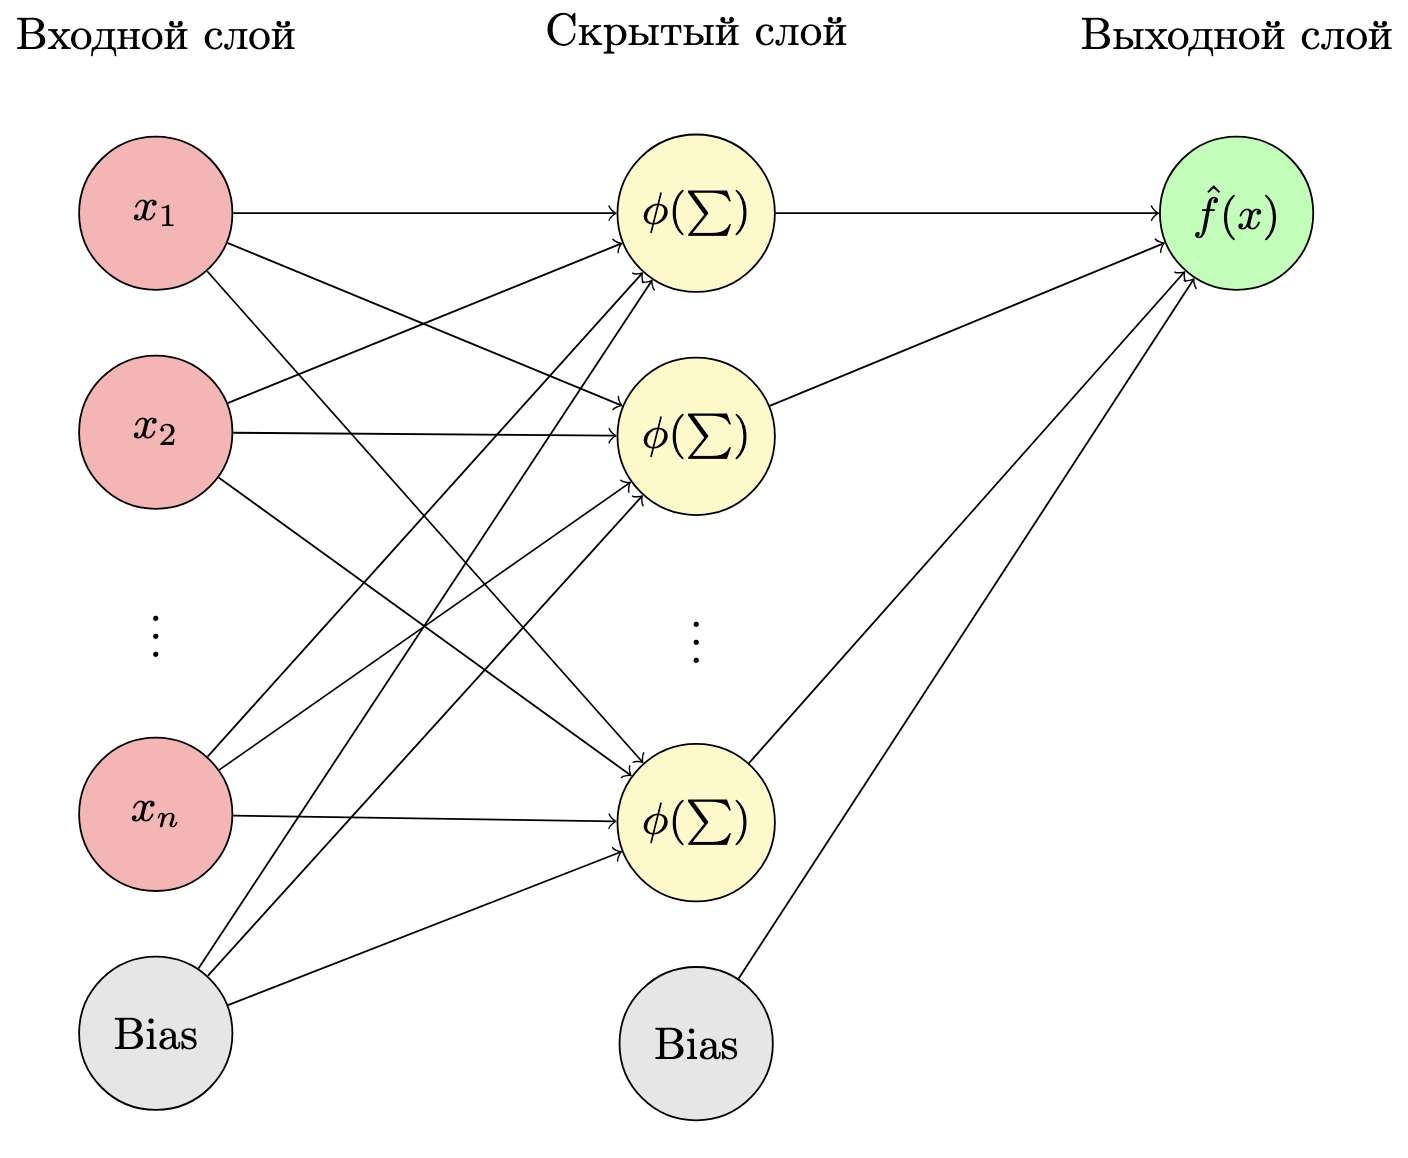
\includegraphics[width=0.5\linewidth]{architecture.png}
    \caption{Архитектура \textit{MLP} описываемой нейросети}
    \label{fig:enter-label}
\end{figure}

Данный аналитический вид $\hat{f}(x)$, как описано выше, можно интегрировать и на его основе получить формулу численного интегрирования на основе параметров нейросети (1-4). Для интегрирования аналитического вида нейросети (5) можно воспользоваться удобным соответствием логистической сигмоиды полилогарифму нулевого порядка:

\begin{equation}
    -Li_0(-\exp(•)) = \frac{1}{1+\exp(-•)}
\end{equation}

\noindent
который достаточно легко интегрировать аналитически. На основе аналитического интеграла нейросети (5), заменив сигмоиду полилогарифмом, как показано выше (7), можно получить формулы (1-4). Нейросетевой подход, таким образом, сводится к следующим шагам:

\begin{enumerate}
    \item Создание набора данных на основе значений подынтегральной функции и её переменных для обучения нейросетевой модели.
    \item Обучение и тестирование нейросетевой модели (5) аппроксимировать подынтегральную функцию.
    \item Извлечение параметров нейросетевой модели и применение их в формулам (1-4) для получения численного значения интеграла.
\end{enumerate}

\section{Описание физической задачи}

Основная задача: моделирование процессов образования и свойств частиц для эксперимента \textit{NICA}. В рамках задачи необходимо создать модель, описывающую основные свойства как лёгких, так и тяжелых мезонов. Для этого будет использоваться модель с нелокальными взаимодействиями \cite{blaschke2012meson}\cite{costa2003pseudoscalar}.

Суть модели состоит в том, что образование мезонов (как кварк-антикварковых пар) сопровождается обменом глюонов, однако обмен глюонов не описывается с помощью суммирования диаграмм, так как теория возмущений неприменима (разложение по малой константе связи невозможно) (см. рис. 2).
\renewcommand{\figurename}{Рисунок}
\renewcommand{\thefigure}{2}
\begin{figure}[H]
    \centering
    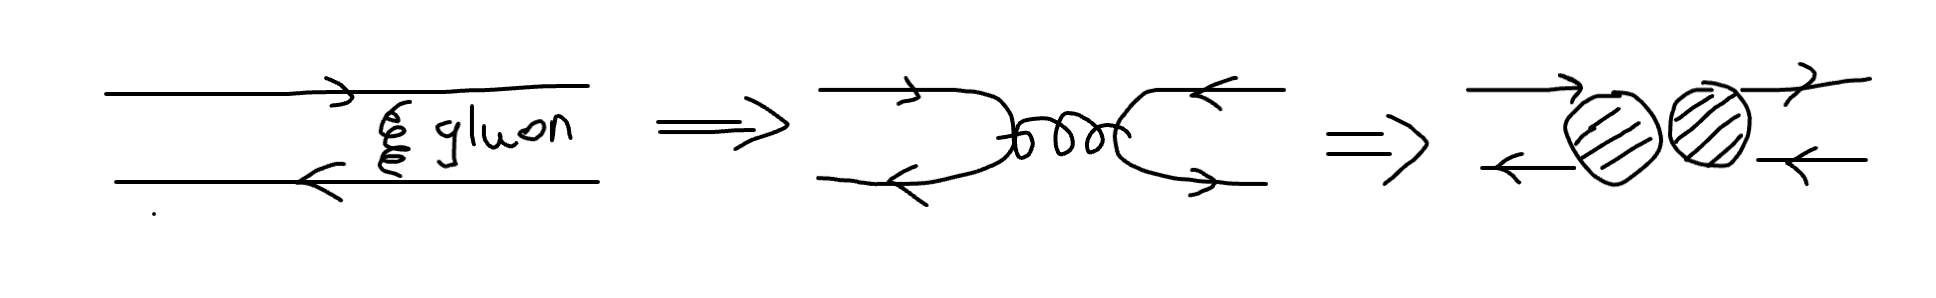
\includegraphics[width=0.5\textwidth]{interaction.png}
    \caption{Взаимодействие с обменом глюонов}
\end{figure}


Назовём \tikz \fill[black] (0,0) circle [radius=1.ex]; форм-фактором и будем использовать модель Гауссовского типа 
\begin{equation}
    F(p^2)=\exp[\frac{-p^2}{\lambda^2}],
\end{equation}
так что размер форм-фактора будет определяться описанной $F(p^2)$. Для описания частиц нам требуется знать массы, константы распадов и процесс распадов. Обозначим взаимодействие:

\begin{figure}[H]
    \centering
    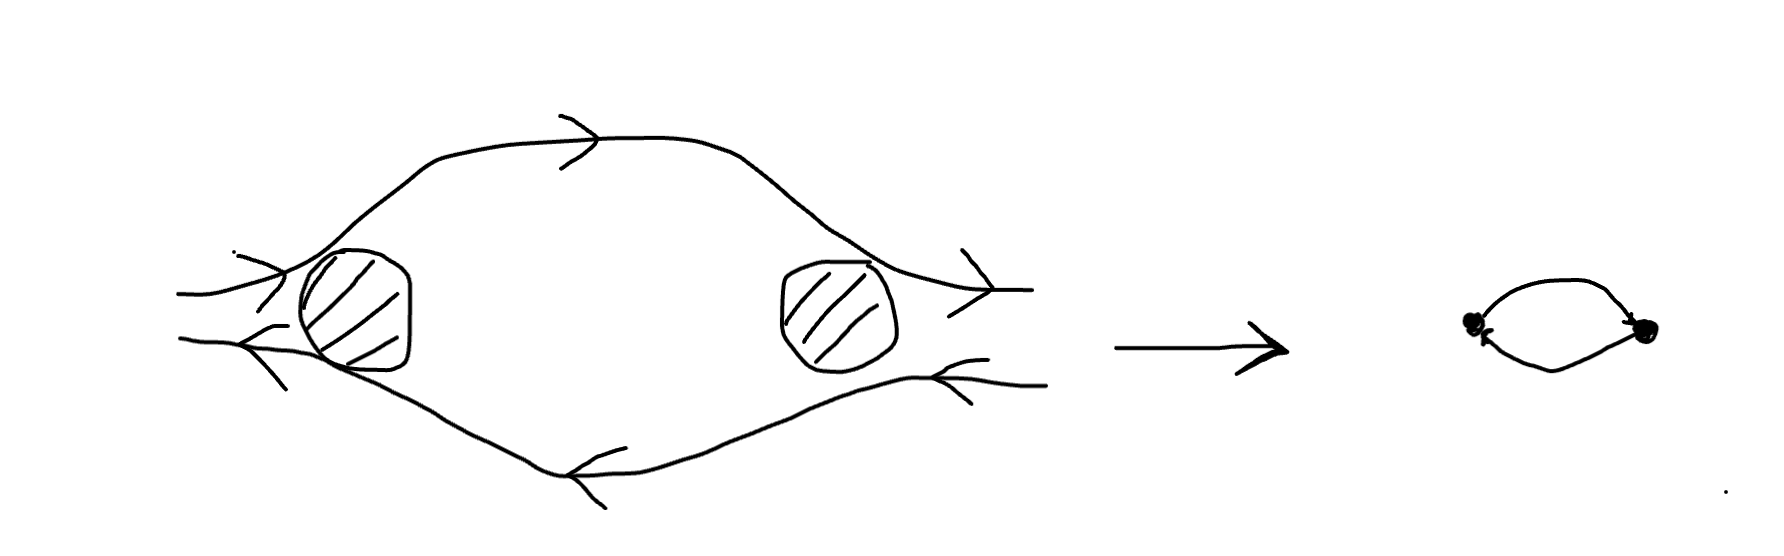
\includegraphics[width=0.5\textwidth]{mases.png}
\end{figure}

и тогда можно выразить:

\begin{equation}
    \tikz[baseline=-0.5ex]{
    \filldraw (0, 0) circle (0.1cm);
    \filldraw (1, 0) circle (0.1cm);
    \draw[->, thick] (0.1, 0.05) to[out=45, in=135] (0.9, 0.05);
    \draw[<-, thick] (0.1, -0.05) to[out=-45, in=-135] (0.9, -0.05);
} + \tikz[baseline=-0.5ex]{
    \filldraw (0, 0) circle (0.1cm);
    \filldraw (1, 0) circle (0.1cm);
    \draw[->, thick] (0.1, 0.05) to[out=45, in=135] (0.9, 0.05);
    \draw[<-, thick] (0.1, -0.05) to[out=-45, in=-135] (0.9, -0.05);
}\tikz[baseline=-0.5ex]{
    \filldraw (0, 0) circle (0.1cm);
    \filldraw (1, 0) circle (0.1cm);
    \draw[->, thick] (0.1, 0.05) to[out=45, in=135] (0.9, 0.05);
    \draw[<-, thick] (0.1, -0.05) to[out=-45, in=-135] (0.9, -0.05);
} + ... = \frac{1}{1 - \tikz[baseline=-0.5ex]{
    \filldraw (0, 0) circle (0.1cm);
    \filldraw (1, 0) circle (0.1cm);
    \draw[->, thick] (0.1, 0.05) to[out=45, in=135] (0.9, 0.05);
    \draw[<-, thick] (0.1, -0.05) to[out=-45, in=-135] (0.9, -0.05);
}}. 
\end{equation}

\begin{equation}
    \tikz[baseline=-0.5ex]{
    \filldraw (0, 0) circle (0.1cm);
    \filldraw (1, 0) circle (0.1cm);
    \draw[->, thick] (0.1, 0.05) to[out=45, in=135] (0.9, 0.05);
    \draw[<-, thick] (0.1, -0.05) to[out=-45, in=-135] (0.9, -0.05);
} \to \int_{0}^{\infty}\frac{dp}{2\pi^4}F(p^2)\frac{1}{u_1u_2} = \int_{0}^{\infty}\frac{dp}{2\pi^4}F(p^2)\frac{1}{[(p + q_1)^2 + m_1^2][(p + q_2)^2 + m_2^2]}.
\end{equation}

Для расчета данных интегралов используются формулы:

\begin{equation}
    \frac{1}{(p + q_1)^2 + m_1^2} = \int_{0}^{\infty}dt\{\exp(-t[(p + q_i)^2 + m_i^2])\} 
\end{equation}
\begin{equation}
    F(p^2) = \int_{0}^{\infty}ds\{\exp(-sp^2)F(s)\} 
\end{equation}

Случаи взаимодействия более чем двух мезонов описываются трех- и четырёхкратными интегралами (см. рис. 3).

\renewcommand{\figurename}{Рисунок}
\renewcommand{\thefigure}{3}
\begin{figure}[H]
    \centering
    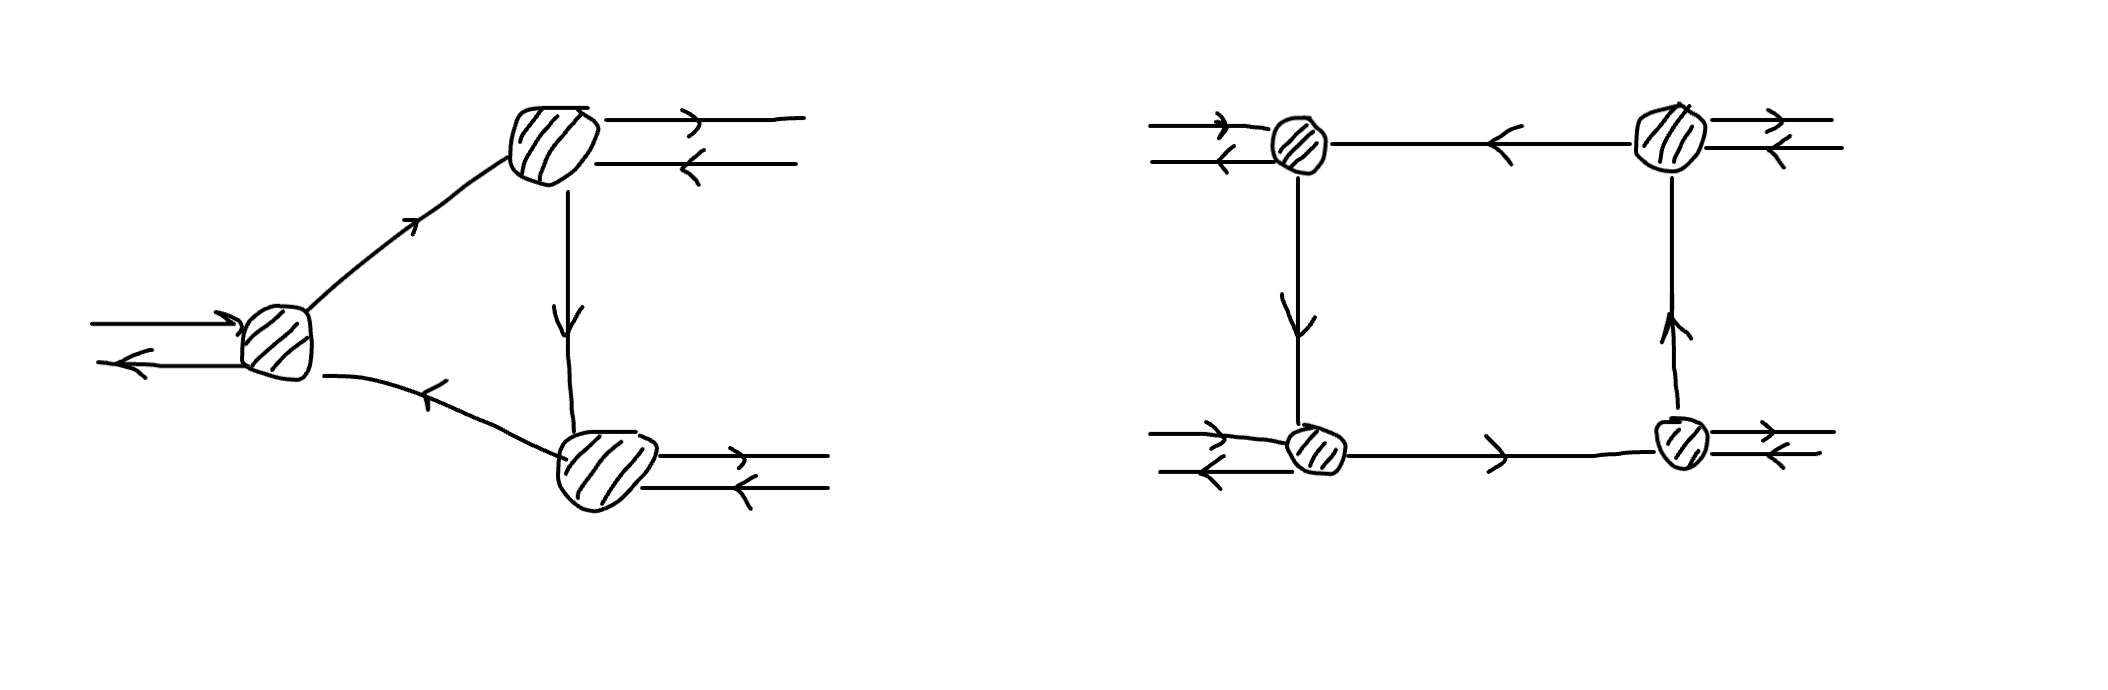
\includegraphics[width=0.5\textwidth]{multiple-interactions.png}
    \caption{Взаимодействие большего числа мезонов}

\end{figure}

Амплитуды конкретных распадов и их квадраты будут вычисляться с помощью программы аналитических вычислений FORM. Основной проблемой данной задачи является исчисление интегралов функций многих переменных.

\section{Применение нейросетевого подхода к физической задаче}

На основе описанного ранее нейросетевого подхода была разработана программная реализация на языке \textit{Python} с применением библиотек \textit{PyTorch}, \textit{NumPy}, \textit{mpmath} \cite{python}\cite{pytorch}\cite{numpy}\cite{mpmath}. В вышеописанной задаче сформулирован повторный интеграл (13), который применяется в различных вычислениях в рамках задачи. Данный интеграл был одним из способов тестирования работоспособности разрабатываемого нейросетевого подхода.

\begin{equation}
    \int_{0}^{1}d\alpha\{\alpha^{a}(1 - \alpha)^b\}\int_{0}^{\infty}dt\{\frac{t^m}{(1+t)^n}F[z_{0}]\} \equiv I(a, b, m, n; F[z_{0}]),
\end{equation}
\begin{equation}   
    F[z_0] = \exp[-2z_0],
\end{equation}
\begin{equation} 
    z_0 = tD + \frac{t}{1 + t}R^2,
\end{equation}
\begin{equation}     
    D = \alpha_1(b_1^{2}P^2 + m_1^2) + \alpha_2(b_2^{2}P^2 + m_2^2),
\end{equation}
\begin{equation} 
        R^2 = (\alpha_1^{2}b_1^2 + \alpha_2^{2}b_2^2 + 2\alpha_{1}\alpha_{2}b_{1}b_2)P^2,
\end{equation}
\begin{equation} 
    b_1 = -\frac{m_1}{m_1 + m_2},
\end{equation}
\begin{equation} 
    b_2 = \frac{m_2}{m_1 + m_2}.
\end{equation}

Предварительно, с использованием языка \textit{FORTRAN}, были получены значения выражения (13) с различными параметрами $a$, $b$, $m$, $n$. Также, для  выражения (13) заданы неизменные значения $m_1 = m_2 = 0.7083333, P^2 = -1.665046$. 

На первом этапе тестирования были вычислены интегралы по $d\alpha$ и по $dt$ по отдельности. Точное значение интеграла функции $\alpha^{a}(1 - \alpha)^b$ было легко получить аналитически, поэтому имелась возможность сравнивать значения, получаемые с использованием нейросетевого подхода и точные значения. Точное значение интеграла $\frac{t^m}{(1+t)^n}F[z_{0}]$ получить было сложнее, поэтому в данном случае акцент был на значение функции потерь \textit{MSE} на тестовом наборе данных для данного интеграла.

На втором этапе тестирования была предпринята попытка интегрирования выражения (13) по двум переменным. Для этого было выполнено следующее преобразование повторного интеграла:

\begin{equation}
 \int_{0}^{1} \alpha^{a}(1 - \alpha)^bd\alpha \int_{0}^{\infty}\frac{t^m}{(1+t)^n}F[z_{0}]dt = 
 \int_{0}^{1} \int_{0}^{\infty}\frac{t^m}{(1+t)^n}F[z_{0}]\alpha^{a}(1 - \alpha)^bdtd\alpha .
\end{equation}

Это позволило обучить нейросетевую модель аппроксимировать функцию $\frac{t^m}{(1+t)^n}F[z_{0}]\alpha^{a}(1 - \alpha)^b$ как функцию двух переменных и воспользоваться нейросетевым подходом для получения значения численного интеграла (13).

РЕЗУЛЬТАТЫ

\section{Заключение и дальнейшие планы}

В настоящее время ведется работа над программной реализацией нейросетевого подхода для функций двух и более переменных, которые будут апробированны на более сложных выражениях из задачи описания свойств мезонов, включающих интегралы функций двух и более переменных. Финальной целью данной работы должен стать программный пакет на языке \textit{Python}, позволяющий применять нейросетевой подход для интегрирования сложных функций как в данной задаче, так и в других задачах как теоретических, так и прикладных.

\printbibliography[
heading=bibintoc,
title={Список литературы}
]
\end{document}